%ATC_example
\begin{figure}[t]
\centering
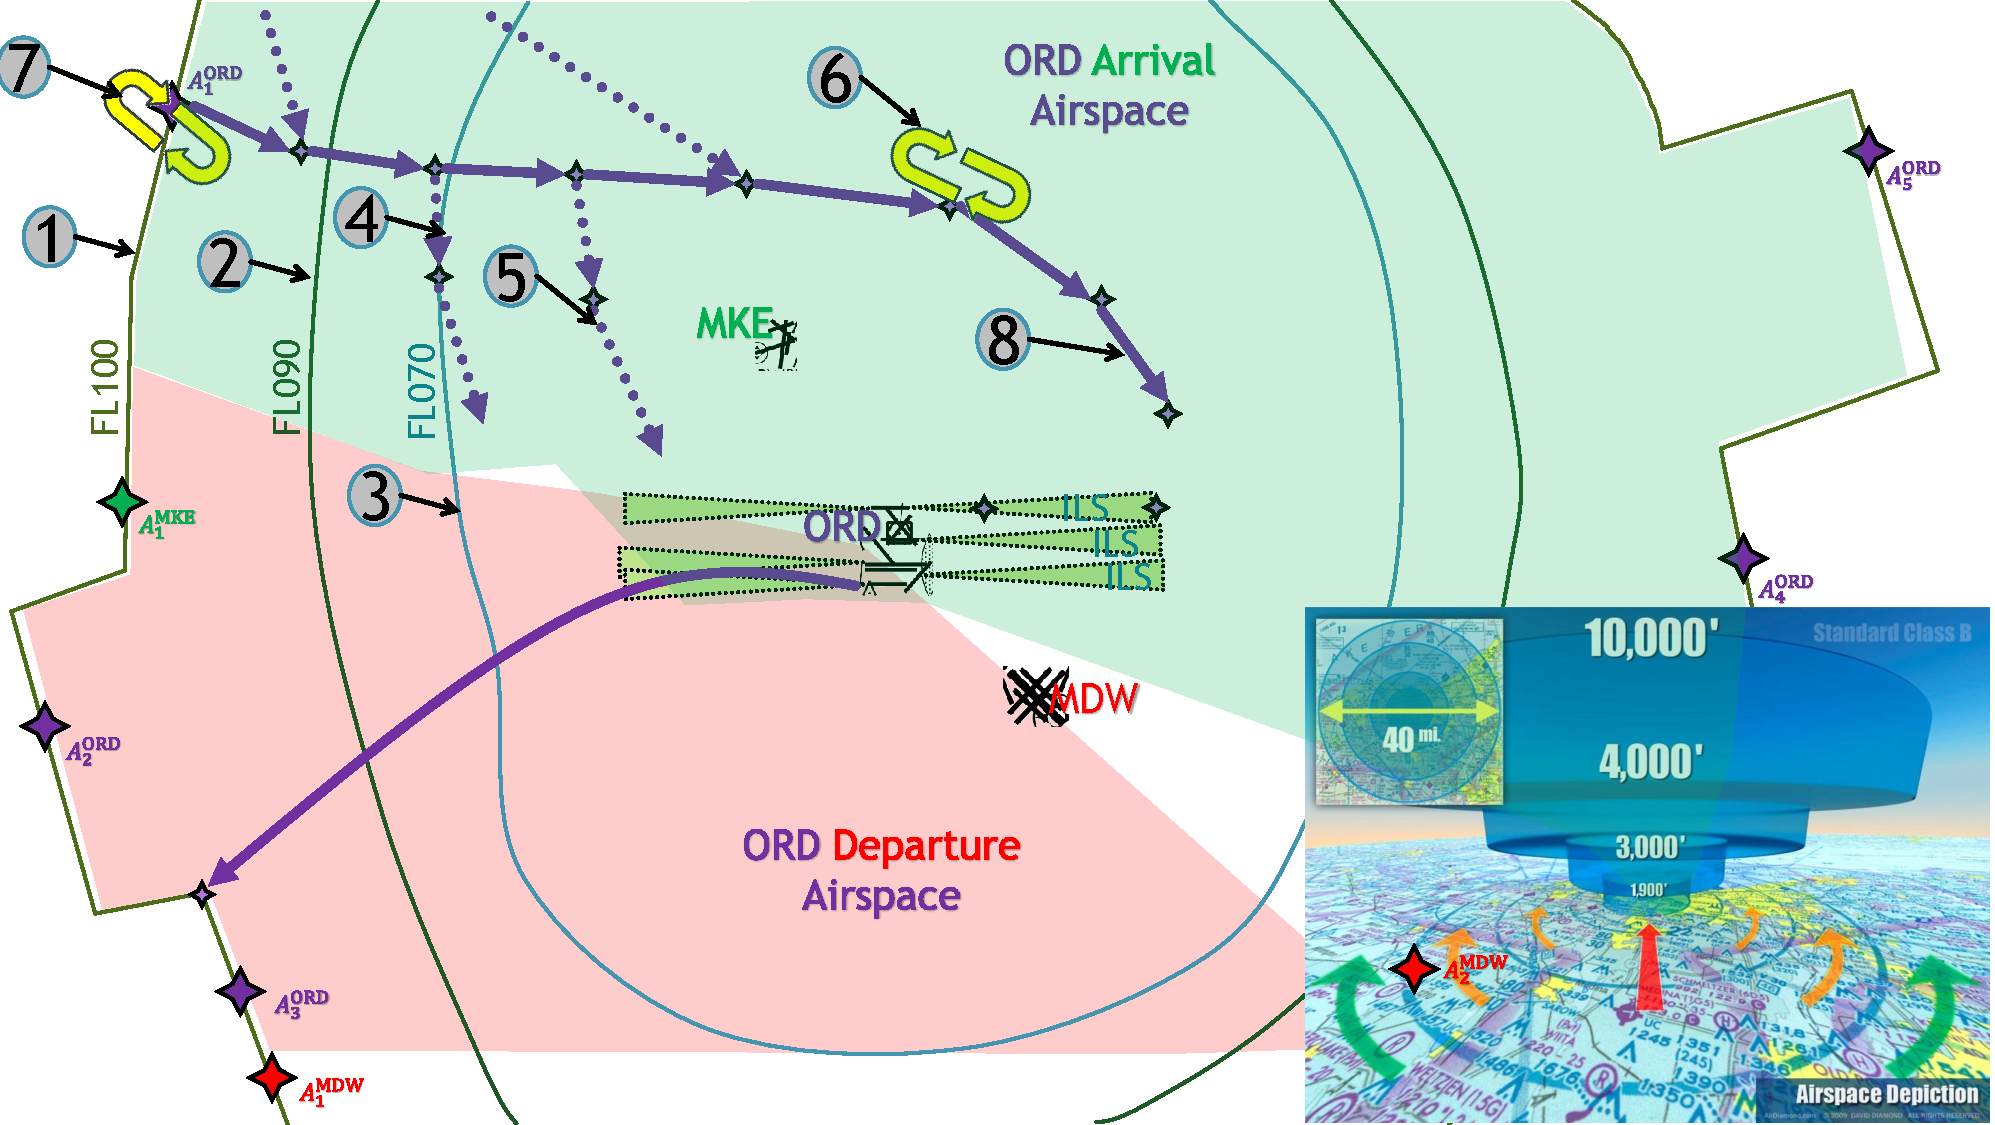
\includegraphics[width=0.49\textwidth]{figures/ATC_Example}
%\vspace{-10pt}
\caption{{\small A simplified depiction of Chicago O'Hare (ORD) airport and its airspace (40 miles radius). The numbers indicate when and where different landing rules apply. Sub-figure on the right shows the altitude rules, see text. Figure courtesy of Max Z. Li, University of Pennsylvania.}} 
		%\todo[inline]{Yash, double-check what i wrote in the caption. what is that sub-figure on the right?}}
\label{fig:atc_example}
%\vspace{-20pt}
\end{figure}

\begin{exmp}
\label{ex:ATC_example}
%{\sf Example 1: Air Traffic Control}.
Air-Traffic Control (ATC) coordinates landing arrivals at an airport. 
ATCs have very complex rules to ensure that all airplanes, of different sizes and speeds, approach the airport and land safely, \textit{with sufficient margin to other airplanes} to accommodate emergencies and wind gusts.
Fig. \ref{fig:atc_example} depicts the airspace of Chicago O'Hare (ORD), the third busiest airport in the U.S.
The arrival airspace is divided into 3 zones with different, hierarchical, altitude floors and ceilings. 
It also shows holding zones, landing approaches, and allowable trajectories for the landing. 
The following is a subset of the rules that apply for incoming air-crafts.

\begin{enumerate}
\vspace{-1pt}
\item When an aircraft enters one of the zones (indicated by the numbers 1,2,3 in Fig.~\ref{fig:atc_example}), it must stay between that zone's altitude floor and ceiling.% E.g. zone 1 has a ceiling of 10,000 feet and a floor of 4000 feet.
\label{rule:floor ceiling}
% of has $1$, $2$ and $3$ mark three Zones, FL100, FL90 and FL70 with altitude ceilings of $10000$, $9000$ and $7000$ feet, and floors of $4000$, $3000$ and $1900$ feet respectively.
\vspace{-1pt}
\item If an aircraft approaches from the West, it must follow one of the trajectories numbered $4$ or $5$. 
%If it approaches from the East (e.g.,  in case of adverse weather), it must follow trajectory $8$.
\label{rule:waypoints}
\vspace{-1pt}
\item If the air-space is too busy, an aircraft must maintain a holding pattern in either holding zones $6$ or $7$, until some maximum amount of time expires.
\label{rule:holding}
% show two holding zones, one at the outer Zone (FL100) and the other in the inner-most zone (FL70). An air-craft could be assigned to a holding zone in case the air-space is too busy.
\vspace{-1pt}
\item A minimum separation must be maintained between aircrafts.
\vspace{-1pt}
\end{enumerate}
\end{exmp}
%\begin{flushright} $\blacksquare$ \end{flushright}